\documentclass{beamer}

\newcommand{\course}{CS 1331 Introduction to Object Oriented Programming}
\newcommand{\lesson}{Debugging}
\newcommand{\code}{http://www.cc.gatech.edu/~simpkins/teaching/gatech/cs1331/code}

\author[Chris Simpkins]
{Christopher Simpkins \\\texttt{chris.simpkins@gatech.edu}}
\institute[Georgia Tech] % (optional, but mostly needed)

\date{}


\newcommand{\course}{Introduction to Object-Oriented Programming}
\subject{\course}
\title[\lesson]{\course}
\subtitle{\lesson}

\author[CS 1331]
{Christopher Simpkins \\\texttt{chris.simpkins@gatech.edu}}
\institute[Georgia Tech]

\date[]{}

\newcommand{\link}[2]{\href{#1}{\textcolor{blue}{\underline{#2}}}}
\newcommand{\code}{http://www.cs1331.org/code}

\usepackage{colortbl}

% If you have a file called "university-logo-filename.xxx", where xxx
% is a graphic format that can be processed by latex or pdflatex,
% resp., then you can add a logo as follows:

% \pgfdeclareimage[width=0.6in]{coc-logo}{cc_2012_logo}
% \logo{\pgfuseimage{coc-logo}}

\mode<presentation>
{
  \usetheme{Berlin}
  \useoutertheme{infolines}

  % or ...

 \setbeamercovered{transparent}
  % or whatever (possibly just delete it)
}

\usepackage{tikz}
% Optional PGF libraries
\usepackage{pgflibraryarrows}
\usepackage{pgflibrarysnakes}
\usepackage{pgfplots}
\usepackage{fancybox}
\usepackage{listings}
\usepackage{hyperref}
\hypersetup{colorlinks=true,urlcolor=blue}
\usepackage[english]{babel}
% or whatever

\usepackage[latin1]{inputenc}
% or whatever

\usepackage{times}
\usepackage[T1]{fontenc}
% Or whatever. Note that the encoding and the font should match. If T1
% does not look nice, try deleting the line with the fontenc.


\usepackage{listings}

% "define" Scala
\lstdefinelanguage{scala}{
  morekeywords={abstract,case,catch,class,def,%
    do,else,extends,false,final,finally,%
    for,if,implicit,import,match,mixin,%
    new,null,object,override,package,%
    private,protected,requires,return,sealed,%
    super,this,throw,trait,true,try,%
    type,val,var,while,with,yield},
  otherkeywords={=>,<-,<\%,<:,>:,\#,@},
  sensitive=true,
  morecomment=[l]{//},
  morecomment=[n]{/*}{*/},
  morestring=[b]",
  morestring=[b]',
  morestring=[b]""",
}

\usepackage{color}
\definecolor{dkgreen}{rgb}{0,0.6,0}
\definecolor{gray}{rgb}{0.5,0.5,0.5}
\definecolor{mauve}{rgb}{0.58,0,0.82}

% Default settings for code listings
\lstset{frame=tb,
  language=scala,
  aboveskip=2mm,
  belowskip=2mm,
  showstringspaces=false,
  columns=flexible,
  basicstyle={\scriptsize\ttfamily},
  numbers=none,
  numberstyle=\tiny\color{gray},
  keywordstyle=\color{blue},
  commentstyle=\color{dkgreen},
  stringstyle=\color{mauve},
  frame=single,
  breaklines=true,
  breakatwhitespace=true,
  keepspaces=true
  %tabsize=3
}


% \beamerdefaultoverlayspecification{<+->}


\begin{document}

\begin{frame}
  \titlepage
\end{frame}


%------------------------------------------------------------------------
\begin{frame}[fragile]{Bug}

\begin{center}
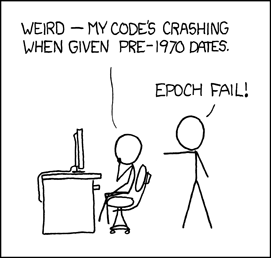
\includegraphics[height=2.5in]{bug.png}\\
\link{http://xkcd.com/376/}{http://xkcd.com/376/}
\end{center}

\end{frame}
%------------------------------------------------------------------------



%------------------------------------------------------------------------
\begin{frame}[fragile]{Program Errors}


Three kinds of program errors, or bugs:
\begin{itemize}
\item Compile-time errors - compiler reports errors and does not produce a .class file
\item Runtime errors - caught by the java runtime
\item Semantic errors - program doesn't do what you expected it to do
\end{itemize}
\vspace{.2in}
BTW, why do we call program errors ``bugs?''

\end{frame}
%------------------------------------------------------------------------

%------------------------------------------------------------------------
\begin{frame}[fragile]{Compile-time Errors}


Java catches many kinds of errors at compile-time, including:
\begin{itemize}
\item Syntax errors - missing semicolons, parenthesis,
\item File name conventions - file name doesn't match name of top-level class in file
\item Type compatibility - a value is assigned to a variable that is not type compatible
\item Name resolution - program refers to a name that is not in scope
\item Method parameter matching - passing the wrong number or type of arguments to a method
\end{itemize}

\end{frame}
%------------------------------------------------------------------------

%------------------------------------------------------------------------
\begin{frame}[fragile]{Runtime Errors}


A program can compile successfully and fail at runtime.
\begin{itemize}
\item Invalid casts - casting a value to an incompatible type
\item Array index out of bounds - referencing an array element with a negative index or an index $\ge$ the array length
\item {\tt NullPointerException} - calling a method or accessing an instance member on an object reference that is {\tt null}
\end{itemize}

\end{frame}
%------------------------------------------------------------------------

%------------------------------------------------------------------------
\begin{frame}[fragile]{Finding Errors}


The process of finding errors is called {\bf debugging}.

\begin{itemize}
\item Fixing compile-time errors is largely a matter of knowing the language and having a keen eye for typos
\item Simple runtime errors, like array indexes out of bounds, are caught and reported with their precise location
\item Semantic errors (which sometimes manifest as runtime errors) require a great deal of patience, detective work, and a toolbag of debugging techniques to find and fix
\end{itemize}

Finding semantic errors comprises the majority of debugging activity.

\end{frame}
%------------------------------------------------------------------------


%------------------------------------------------------------------------
\begin{frame}[fragile]{Debugging Techniques}


Eliminating compile errors is usually called ``getting the code to compile.''  When we talk about debugging we usually mean finding semantic errors.  Some techniques:
\begin{itemize}
\item Tracing and watching - the biggest hammer in the debugging tool bag
\item Assertions
\item Explaining to a colleague, or ``rubber ducking''\footnote{\url{http://c2.com/cgi/wiki?RubberDucking}, \url{http://en.wikipedia.org/wiki/Rubber_duck_debugging}}
\end{itemize}

\end{frame}
%------------------------------------------------------------------------

%------------------------------------------------------------------------
\begin{frame}[fragile]{Tracing and Watching}


Tracing the flow of execution of code can help to locate a bug.
\begin{itemize}
\item Manual: Print statements and logging give a play-by-play report of a program run
\item Debugger: Breakpoints in a debugger allow you to step through a running program one statement at a time
\end{itemize}

Tracing is usually combined with watching the values of variables as the program runs
\begin{itemize}
\item Manual: Print statements and logging include values of variables of interest
\item Debugger: variables can be designated as ``watch'' variables and be displayed separately while the program runs
\end{itemize}

Let's try some of these techniques on \link{\code/Bugs.java}{Bugs.java}

\end{frame}
%------------------------------------------------------------------------

%------------------------------------------------------------------------
\begin{frame}[fragile]{Assertions}


Assertions are statements about program conditions that should be true at a given point of program execution.
\begin{lstlisting}[language=Java]
assert condition;
\end{lstlisting}
\vspace{-.1in}
\begin{itemize}
\item {\tt condition} is any boolean expression
\item Normally, assertions are not checked
\item To hava {\tt java} check assertions, run program with {\tt enableassertions} switch
\item A more robust version of {\tt \#IFDEF DEBUG} from the old C days
\end{itemize}
With {\tt enableassertions} switch, when some {\tt condition} in an assertion is {\tt false}, the program terminates with a {\tt java.lang.AssertionError}.

\vspace{.1in}
Assertions are useful for checking semantic errors in your programs, but require some effort.


\end{frame}
%------------------------------------------------------------------------

%------------------------------------------------------------------------
\begin{frame}[fragile]{Insertion Sort}


The insertion sort algorithm in pseudocode (from CLRS Chapter 2):
\vspace{-.05in}
\begin{lstlisting}[]
1 for j = 2 to A.length // A[1 .. A.length] is an array
2     key = A[j]
3     // Insert A[j] into the sorted sequence A[i .. j - 1].
4     i = j - 1
5     while i > 0 and A[i] > key
6         A[i + 1] = A[i]
7         i = i - 1
8    A[i + 1] = key
\end{lstlisting}

Insertion sort implemented in Java:
\vspace{-.05in}
\begin{lstlisting}[language=Java]
for (int j = 1; j < a.length; ++j) {
    int key = a[j];
    int i = j - 1;
    while(i >= 0 \&\& a[i] > key) {
        a[i + 1] = a[i];
        i = i - 1;
    }
    a[i + 1] = key;
}
\end{lstlisting}

\end{frame}
%------------------------------------------------------------------------

%------------------------------------------------------------------------
\begin{frame}[fragile]{Loop Invariants}


A loop invariant expresses a formal property of an algorithm that:
\begin{itemize}
\item is true prior to the first iteration of the loop,
\item if it is true before an iteration of the loop remains true before the next iteration, and
\item upon loop termination gives a useful property that helps show that the algorithm is correct.
\end{itemize}


\end{frame}
%------------------------------------------------------------------------

%------------------------------------------------------------------------
\begin{frame}[fragile]{A Loop Invariant for Insertion Sort}

\begin{lstlisting}[]
1 for j = 2 to A.length
2     key = A[j]
3     // Insert A[j] into the sorted sequence A[1 .. j - 1].
4     i = j - 1
5     while i > 0 and A[i] > key
6         A[i + 1] = A[i]
7         i = i - 1
8    A[i + 1] = key
\end{lstlisting}

\begin{quote}
At the start of each iteration of the for loop of lines 1-8, the subarray A[1 .. j - 1] consists of the elements originally in A[i .. j - 1], but in sorted order.
\end{quote}

\end{frame}
%------------------------------------------------------------------------


%------------------------------------------------------------------------
\begin{frame}[fragile]{Expresing Loop Invariants as {\tt assert}ions}


Translating the assertion condition is easy.  The trick is figuring out where to put it.

\begin{lstlisting}[language=Java]
for (int j = 1; j < a.length; ++j) {
    assert isSorted(a, 0, j - 1);
    int key = a[j];
    int i = j - 1;
    while(i >= 0 \&\& a[i] > key) {
        a[i + 1] = a[i];
        i = i - 1;
    }
    a[i + 1] = key;
}
\end{lstlisting}
Note that we didn't express the entire invariant in Java.  We could, but you must trade off implementation effort and benefit. Run the program with the {\tt -ea} switch to enable assertions:
\begin{lstlisting}[language=Java]
$ java -ea InsertionSort
\end{lstlisting}

See \link{\code/algorithms-code/InsertionSort.java}{InsertionSort.java}.


\end{frame}
%------------------------------------------------------------------------

%------------------------------------------------------------------------
\begin{frame}[fragile]{Avoiding Bugs}

\begin{quote}
There are two ways to write error-free programs; only the third one works. -- Alan Perlis
\end{quote}

\begin{itemize}
\item Defensive programming - validate input, check array bounds, check for nulls, use checked expections
\item Incremental development - develop program in small pieces, test peices individually before combining
\item Code review/pair programming - have another set of eyes on your code
\end{itemize}

\vspace{.2in}
Let's add some defensive code to \link{\code/Bugs.java}{Bugs.java}

\end{frame}
%------------------------------------------------------------------------



%------------------------------------------------------------------------
\begin{frame}[fragile]{Closing Thoughts}


\begin{itemize}
\item Computers are compliant and finicky
\item Debugging is an art and a science
\item Think like a detective
\item Code defensively
\end{itemize}


\end{frame}
%------------------------------------------------------------------------


\end{document}
